%% Requires compilation with XeLaTeX or LuaLaTeX
\documentclass[10pt,xcolor={table,dvipsnames},t]{beamer}
\usetheme[background=dark]{trigon}
\usepackage{amsmath}
\usepackage{nicefrac}
\usepackage{amssymb}
%\usepackage{enumitem}
\usepackage{braket}
\usepackage{empheq}
\usepackage{color}
\usepackage{keyval}
\usepackage{subcaption}
\usepackage{calrsfs}
\usepackage{hyperref}
\usepackage{eufrak}
\usepackage{transparent}
\usepackage{tikz}
\usepackage{nicematrix}
\usepackage{setspace}

\captionsetup{font=scriptsize}
\title{Open Quantum System}
\subtitle{
  Lectures: \\ 
  \footnotesize
  \begin{itemize}
      \setlength\itemsep{-0.5em}
    { 
      \transparent{0.4}
    \item[] Last time:
    \item Daniel Manzano, A short introduction to the Lindblad master equation (\textit{all})
    \item Breuer and Petruccione, The Theory of Open Quantum Systems (\textit{ch. 3 - 4.3})
    \item Daniel A. Lidar, Notes on the Theory of Open Quantum Systems (\textit{up to ch. 12})
    }
  \item[] Today:
    \item Buča, B., Tindall, J. \& Jaksch, D. Non-stationary coherent quantum many-body dynamics through dissipation
    \item Victor V. Albert \& Liang Jiang, Symmetries and conserved quantities in Lindblad master equations
    \item Cameron Booker, Berislav Buča, Dieter Jaksch, Non-stationarity and Dissipative Time Crystals: Spectral Properties and Finite-Size Effects
    \item Victor V. Albert. Lindbladians with multiple steady states: 
      theory and applications. A Dissertation Presented to the Faculty of the Graduate School of Yale University
  \end{itemize}
  \vspace{-1cm}
}
\newcommand{\dt}{\frac{d}{dt}}
\newcommand{\lan}{\mathcal{L}}
\newcommand{\Hint}{H_{\text{int}}}
\newcommand{\outerprod}[2]{\ket{#1}\!\!\bra{#2}}
\newcommand{\outerprodd}[3]{\ket{#1}\!_{#2}\!\bra{#3}}
\newcommand{\tr}[2]{\text{Tr}_{#1}\bigl[#2\bigr]}
\newcommand{\kett}[1]{\vert #1 \rangle\!\rangle}
\newcommand{\circledmathfrak}[1]{
  \tikz[baseline=(char.base)]{
    \node[shape=circle,draw,inner sep=2pt] (char) {$\mathfrak{#1}$};
  }
}


\setbeamertemplate{footline}{
  \hbox{%
    \begin{beamercolorbox}[wd=.5\paperwidth,ht=2.5ex,dp=1ex,left]{author in head/foot}%
      %\usebeamerfont{author in head/foot}\insertshortauthor~~(\insertshortinstitute)
    \end{beamercolorbox}%
    \begin{beamercolorbox}[wd=.5\paperwidth,ht=2.5ex,dp=1ex,right]{title in head/foot}%
    \end{beamercolorbox}}%
  \vskip0pt%
}

\newlength\mytemplen
\newsavebox\mytempbox
\usepackage{accents}
\newlength{\dhatheight}

\newcommand{\doublehat}[1]{%
    \settoheight{\dhatheight}{\ensuremath{\hat{#1}}}%
    \addtolength{\dhatheight}{-0.15ex}%
    \hat{\vphantom{\rule{1pt}{\dhatheight}}%
    \smash{\hat{#1}}}}

\newcommand\mybluebox{%
    \@ifnextchar[%]
       {\@mybluebox}%
       {\@mybluebox[0pt]}}

\definecolor{myblue}{rgb}{.8, .8, 1}

\def\@mybluebox[#1]{%
    \@ifnextchar[%]
       {\@@mybluebox[#1]}%
       {\@@mybluebox[#1][0pt]}}

\def\@@mybluebox[#1][#2]#3{
    \sbox\mytempbox{#3}%
    \mytemplen\ht\mytempbox
    \advance\mytemplen #1\relax
    \ht\mytempbox\mytemplen
    \mytemplen\dp\mytempbox
    \advance\mytemplen #2\relax
    \dp\mytempbox\mytemplen
    \colorbox{myblue}{\hspace{1em}\usebox{\mytempbox}\hspace{1em}}}

\newcommand{\Nwarrow}{\rotatebox[origin=c]{135}{\(\Longleftrightarrow\)}}
\newcommand{\Nwarrowl}{\rotatebox[origin=c]{225}{\(\Longleftrightarrow\)}}

\begin{document}

\begin{frame}
  \titlepage
\end{frame}

\begin{frame}{Recalling notations}
  \begin{columns}
    \begin{column}{0.5\textwidth}
      Assumption \circledmathfrak{a}: 
      \begin{center}
      $\forall \omega\; \exists ! \{m,n\}: e_m- e_n = \omega$
    \end{center}
    This implied that $\mathcal{H}_S = \text{span}(\outerprodd{m}{\omega}{n})$
    \begin{figure}
      \centering
      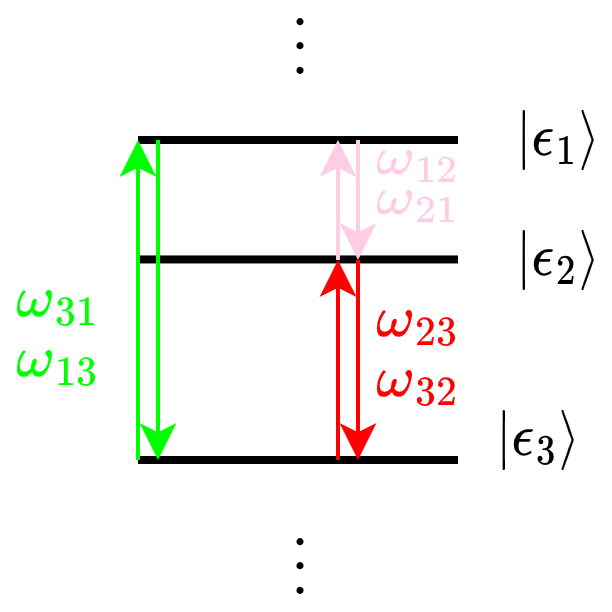
\includegraphics[width=0.8\textwidth]{./energy_levels.png}
    \end{figure}
    \end{column}
    \begin{column}{0.5\textwidth}
      Assumption \circledmathfrak{b}:\\
      \begin{center}
      \circledmathfrak{a} + 1 degeneracy of order 1
    \end{center}
    \begin{center}
    \begin{figure}
      \centering
      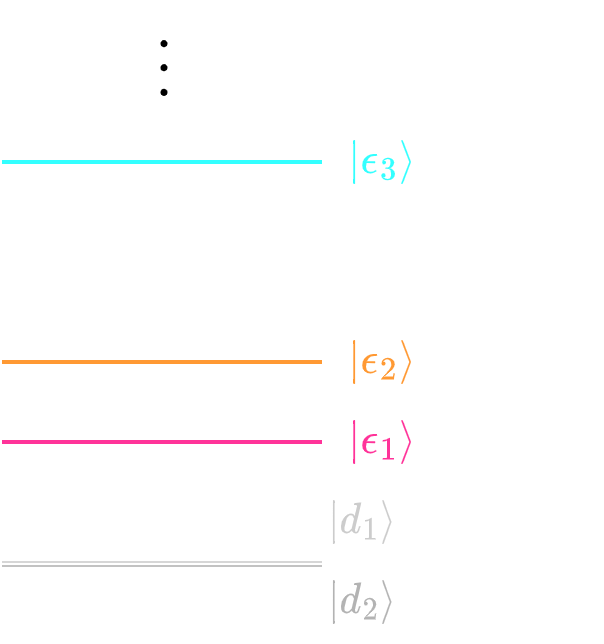
\includegraphics[width=0.7\textwidth]{./energy_levels_deg1.png}
    \end{figure}
  \end{center}
    \end{column}
  \end{columns}
\end{frame}

\begin{frame}{}
  \begin{block}{Conditions on $A$ - assumption \circledmathfrak{a}}
    \begin{itemize}
      \item<1-> Last time derivation - 
        $$
        \bigl[ \outerprodd{m}{\omega}{m} L_\nu^{(\dag)} \outerprodd{n}{\omega}{n}, A \bigr] = 0\quad \text{ with } A= \sum_{kl}a_{kl}\outerprod{k}{l}
        $$
      \item<2-> Is it true that $A = \lambda \mathbb{I}$ \;i.e.\; $\ket{m} \neq \ket{n} \overset{?}{\implies} a_{mn} = 0$
      \item<3-> Relations from last time:
        \begin{gather}
          \begin{rcases}
          a_{nm} \langle m \vert L_\nu \vert n \rangle = 0 \;, \quad a_{mn} \langle n \vert L_\nu ^\dag \vert  m \rangle = 0 \\
          \begin{cases}
          a_{nn}\langle m \vert L_\nu \vert n \rangle = a_{mm} \langle m \vert L_\nu \vert n\rangle \\
          a_{nn}\langle n \vert L_\nu^\dag \vert m \rangle = a_{mm} \langle n \vert L_\nu^\dag \vert m\rangle 
        \end{cases}
      \end{rcases}
           \qquad\forall \{m, n, \nu\} 
      \end{gather}
    \item<4->[] \begin{center}Question - does this imply that $a_{mn} = 0$?\end{center}
    \item<4->[] \begin{center}Since from def. of $L_\nu$ - $H_{\text{int}} = \sum_\nu S_\nu \otimes B_\nu$\;,\;\; with 
      $L_\nu \overset{\mathsf{u}}{\sim} S_\nu$\;? \end{center}
    \end{itemize}
  \end{block}
\end{frame}
\begin{frame}{Conditions on A}
  \begin{block}{Conditions on $A$ - assumption \circledmathfrak{a}}
    \begin{itemize}
      \item<1-> Thus, condition on $a_{kl}$ depends on whether $L_\nu$ couples $\ket{m}, \ket{n}$\;\; $\forall \nu$?
    \end{itemize}
  \end{block}
  \only<2->{
    \begin{block}{Conclusion #1}
      \begin{center}
      If $\forall \ket{m} \neq \ket{n}$, \; $\exists \nu $\; such that $\bra{m} L_\nu \ket{n} \neq 0$\quad  $\implies$ \quad $A = \lambda \mathbb{I}$
    \end{center}
    Intuitively, $A = \lambda \mathbb{I}$ if $\Hint$ does not couple all $\outerprod{k}{l}$. I.e. if the $\Hint$ is 
    not in the form $\Hint = \sum_{m < n \in \sigma(H_S)} \outerprod{m}{n}\otimes B_{m,n}$.
    \end{block}
  }
  \only<3->{
    \begin{block}{Conclusion #2}
      \begin{center}
        If $\exists m\neq n$ \; such that $\forall \nu$, \, $\bra{m}L_\nu \ket{n} = 0$ \; $\implies$ \; 
        $A \neq \lambda \mathbb{I}$
      \end{center}
    \end{block}
  }
\end{frame}


\begin{frame}
  \begin{block}{Conditions on $A$ - assumption \circledmathfrak{b}}
    \begin{itemize}
      \item<1->[] Obtained relation from last time for assumption \circledmathfrak{b}:
        \begin{align}
          a_{aa} \bra{b} L_\nu \ket{a} = a_{bb} \bra{b} L_\nu \ket{a} \notag \\
          a_{aa} \bra{a} L_\nu \ket{b} = a_{bb} \bra{a} L_\nu \ket{b} \notag \\
          a_{ab} \bra{b} L_\nu \ket{a} = a_{ba} \bra{a} L_\nu \ket{b} \notag 
        \end{align}
      \item<2->[] Then, for some non-degenerate $\ket{g}$ 
        \begin{align}
          a_{ag} \bra{g} L_\nu \ket{a} = a_{ag}\bra{g}L_\nu \ket{b} = 0 \notag \\
          a_{bg} \bra{g} L_\nu \ket{a} = a_{bg}\bra{g} L_\nu \ket{b} = 0 \notag 
        \end{align}
      \item<3->[] And additional relations 
        \begin{align}
          a_{aa} \bra{g} L_\nu \ket{a} + a_{ba} \bra{g} L_\nu \ket{b} = a_{gg} \bra{g} L_\nu \ket{a} \notag 
        \end{align}
        \vspace{-0.75cm}
        $$
        ...
        $$
    \end{itemize}
  \end{block}
\end{frame}


\begin{frame}{}
  \only<1->{
  \begin{block}{Conclusions on $A$ under \circledmathfrak{b}}
  One can write the form of $A$ 
$$
\begin{pNiceArray}{cc|ccc}
  \Block{2-2}<\Large>{\mathbf{A^*_0}}& & \ddots & * & \ddots \\
                                    && * & \ddots & * \\
  \hline
  \ddots & * & \Block{3-3}<\Large>{\mathbf{\lambda \mathbbm{I}}} \\
  * & \ddots &&& \\
  \ddots & * &&&
\end{pNiceArray}
$$
  \end{block}
  If same conditions on $L_\nu$ (\,$L_\nu \equiv \text{span}(\ket{g}\!\!\bra{a,b})\; \forall \ket{g}$\,), then it is 
  block diagonal with $\mathbf{A_0^*}$ and $\mathbf{\lambda I}$.
}
\end{frame}

\begin{frame}{Examples}
  \begin{itemize}
    \item<1-> Spontaneous emission 
      \begin{gather}
          H_{SB} = g\sum_\nu L_\nu \otimes B_\nu = g\bigl( \outerprod{e}{g}\otimes a + \outerprod{g}{e}\otimes a^\dag \bigr) \notag \\
      L_1 = \outerprod{e}{g} \quad \text{ and } \quad L_2 = \outerprod{g}{e} \notag
    \end{gather}
    \item<2-> If multiple atoms, assumption \circledmathfrak{a} does not hold. (?)
    \item<3-> Spin Chain Coupled to Magnetic Fluctuations - 
      \begin{itemize}
        \item <3-> Heizenberg XY model $H_S = J\sum_i(s_i^x s_{i+1}^x +s_i^y s_{i+1}^y + \Delta s_i^z s_{i+1}^z)$
        \item <3-> Collection of bosonic modes $H_B = \sum_i \omega_i b_i^\dag b_i$
        \item <4-> Interaction $H_{SB} \equiv \sum_{ik}g_{ik}S^+_i \otimes b_k + g_{ik}^* S_i^- \otimes b_k^\dag$
        \item <4-> Jump operators $S^+ \equiv \outerprod{0}{1}$ and $S^- \equiv \outerprod{1}{0}$ for every $i$.
      \end{itemize}
  \end{itemize}
\end{frame}

\begin{frame}{Symmetries \& Conserved quantities}
  \begin{itemize}
    \item<1->[] \textbf{Steady-state:}
    \item<1-> Conserved quantities $J$ generate symmetries $U$
    \item<1-> If $\mathcal{L}$ has no purely imaginary eigenvalues, let $\{M_\nu\}$ of 
      $\mathsf{L}_{ss} \subseteq \mathsf{L}$ such that  
      $$
      \rho_{ss} = \lim_{t \rightarrow \infty} e^{\mathcal{L}t} = \sum_{\nu}\rho_\nu M_\nu \quad \text{with} \qquad \rho_\nu = 
      \tr{}{J_\nu^\dag M_\nu}
      $$

    \item<2->[] \textbf{Oscillating-coherence}
    \item<2-> Oscillating coherence state $\rho_\infty$, such that $\mathcal{L}\rho_\infty = i\lambda \rho_\infty$ or 
      $\lim_{t \rightarrow \infty }e^{\mathcal{L}t}\rho_\infty = e^{i\lambda t}\rho_\infty$
    \item<2-> In that case, the conserved quantities $\widehat{J}$ also oscillate: 
      $$e^{\mathcal{L} ^\dag t} \widehat{J_{\mu, \nu}} = e^{- i\lambda_{\mu, \nu}t}\widehat{J_{\mu, \nu}} $$
  \end{itemize}

\end{frame}

\begin{frame}{Symmetries \& Conserved quantities}
  \begin{itemize}
    \only<1->{
    \begin{theorem}
      The \underline{steady-states}, \underline{steady-state coherences} and \underline{oscillating coherences} form a basis of the $\mathsf{L}$ space.
    \end{theorem}
  }
    \item<2-> For an oscillating coherence, one can write using a basis $\{M_{\nu}\}$ of the $\mathsf{L}_{ss}$, of 
      dimension $D$
      and the basis $\{O_{\mu, \nu}\}$ for the oscillating coherences, 
      \begin{gather}
        \rho_\infty \quad = \underbrace{\sum_{\mu=1}^D \rho_\mu M_\mu}_
        {\text{\parbox{10em}{\setstretch{0.7}\tiny \centering steady-state \; \& \\ steady-state coherence}}}
        + \quad \underbrace{\sum_{\substack{\mu, \nu \\ \mu \neq \nu}} \rho_{\mu, \nu}(t)\; O_{\mu, \nu}}_
        {\text{oscillating coherence}} \\
        \equiv \; \kett{\rho_\infty} \quad =\quad \sum_{\mu=1}^D \rho_\mu \kett{M_\mu} \quad
        + \quad \sum_{\mu \neq \nu} \rho_{\mu, \nu}(t)\; \kett{O_{\mu, \nu}}
      \end{gather}
  \end{itemize}

\end{frame}
\begin{frame}{Symmetries \& Conserved quantities}
  \begin{itemize}
    \item<1->[]
      \begin{center}
      $\rho_\infty = \sum_{\mu=1}^D \rho_\mu M_\mu
        +  \sum_{\mu \neq \nu} \rho_{\mu, \nu}(t)\; O_{\mu, \nu}$
      \end{center}
    \item<1-> With $\rho_{\mu, \nu}(t)$ defined via 
      \begin{gather}
        \rho_{\mu, \nu}(t) = \langle \! \langle\; \widehat{J}_{\mu, \nu} \kett{\rho_\infty} = 
        \tr{}{\widehat{J}_{\mu, \nu}^\dag \, \rho_\infty}\\
      \rho_{\mu, \nu}(t) = e^{i\lambda_{\mu, \nu}t} \langle \! \langle\; \widehat{J}_{\mu, \nu} \kett{\rho_{in}} 
      = e^{i\lambda_{\mu, \nu}t}\tr{}{\widehat{J}_{\mu, \nu}^\dag\, \rho_{in}}
    \end{gather}
  \item<2-> The oscillating coherence via operator $A$: 
    \begin{gather}
      \mathcal{L} (\rho_{ss}) \quad \xrightarrow[\exists A]{[H,A] \rho_{ss} = \lambda A \rho_{ss} \;\& \; \cdots} 
      \quad \mathcal{L} (A\rho_{ss}) = i \lambda A\rho_{ss} \\
      \implies \rho_{\infty} = A\rho_{ss}
    \end{gather}
  \end{itemize}
\end{frame}

\begin{frame}{Symmetries \& Conserved quantities}
  \begin{itemize}
    \item<1-> Applying $\mathcal{L}$ to $\rho_\infty = \sum_{\mu=1}^D \rho_\mu M_\mu
     +  \sum_{\mu \neq \nu} \rho_{\mu, \nu}(t)\; O_{\mu, \nu}$
   \item<2->[]
     \begin{center}
       \begin{gather*}
         \mathcal{L}(\rho_\infty) = \sum_{\mu=1}^D \rho_\mu \mathcal{L}(M_\mu)
         +  \sum_{\mu \neq \nu} \rho_{\mu, \nu}(t)\; \mathcal{L}(O_{\mu, \nu}) \\
      \mathcal{L}(\rho_\infty) = \sum_{\mu \neq \nu} \rho_{\mu, \nu}(t)\; \mathcal{L}(O_{\mu, \nu})
       \end{gather*}
     \end{center}
   \item<3->[]
     \begin{center}
       \begin{gather*}
         i \lambda \rho_{\infty} = \sum_{\mu \neq \nu} \rho_{\mu, \nu}(t) i \lambda_{\mu, \nu} O_{\mu, \nu} \\
         A\rho_{ss} = \sum_{\mu \neq \nu} \frac{\lambda_{\mu, \nu}}{\lambda} \rho_{\mu, \nu}(t)  O_{\mu, \nu}
       \end{gather*}
     \end{center}
  \end{itemize}
\end{frame}

\begin{frame}{Symmetries \& Conserved quantities}
  \begin{itemize}
    \item<1-> It is possible to write $\rho_\infty$ and $\rho_{ss}$ in a more formal form (B. Baumgartner), 
      (V.V. Albert, L. Jiang)
    \item<1-> For example, a block diagonal form
      \begin{center}
        \begin{gather*}
          \rho_{ss} = \bigoplus_\iota \Bigl[ \sum_{\mu, \nu}^{n_\iota} \rho_{\mu, \nu}^{(\iota)}
            \outerprodd{\mu}{\iota}{\nu} \otimes T^{(\iota)}
          \Bigr] \\
          \rho_{\infty}(t) = \bigoplus_\iota \Bigl[
            \sum_{\mu, \nu}^{n_\iota} \rho_{\mu, \nu}^{(\iota)} e^{i\lambda_{\mu, \nu}^{(\iota)} t} \outerprodd{\mu}{\iota}{\nu}
            \otimes T^{(\iota)}
          \Bigr]
        \end{gather*}
      \end{center}
  \end{itemize}
\end{frame}

\end{document}






